\section{Genomics}
The field of genomics is closely related to, yet distinct, from the field of genetics, which itself stems from the work of such seminal figures as Charles Darwin\autocite{originofspecies} and Gregor Mendel\autocite{mendel1865}. While genetics largely focuses on the study of single (or relatively small numbers of) genes - the \emph{genotype}, and how genetic variation and mutation affect the physical traits of a given cell or organism - its \emph{phenotype}, genomics focuses on larger scale events and mechanisms that tend to act on the entirety of an organism's genome, shaping its architecture and ultimately affecting its survival.

\subsection{History of Genomics}
Each living cell is a bio-chemical machine that carries out a number of complex behaviours such as interactions with the surrounding environment, motility, metabolism, and reproduction, that are necessary for its survival and proliferation, based on a genetic program that is encoded within the cell's DNA. The DNA is nominally subdivided into functionally distinct areas known as \emph{genes}. The cell utilizes the program within each gene by first \emph{transcribing} the DNA into an intermediary information-carrier molecule called RNA, and then \emph{translating} this RNA into molecules called \emph{proteins} that are utilized by the cell to carry out the majority of its functions. Understanding and interpretation of the underlying genetic program thus underpins our ability to comprehend the entirety of the different behaviours that each cell undertakes.

The success of this undertaking is contingent, first and foremost, on our ability to effectively read off the information encoded in the DNA, an activity known as \emph{sequencing}. We are able to sequence DNA thanks to the pioneering work of researchers Rosalind Franklin\autocite{franklin1953molecular}, James Watson, and Francis Crick\autocite{watson1953molecular} who first elucidated the physical structure of DNA, then followed by the work of Fred Sanger\autocite{sanger1977dna,sanger1975rapid} who devised the first effective DNA sequencing method. The sequencing method allows us to transform information that is physically encoded on the DNA molecule via a sequence of four distinct types of \emph{basepairs} - Adenine, Cytosine, Guanine, and Thymine into a string stored on a computer using a four-letter alphabet - A,C,T, and G, thus turning DNA interpretation into a digital information processing problem.

While the entire length of the DNA of an organism ranges from several hundred thousand basepairs for simple organisms like viruses and bacteria, to about 3,000,000,000 basepairs for a human, to over 150,000,000,000 for certain plants\autocite{pellicer2010largest} the limitations of Sanger DNA sequencing technology are such that the sequencing machine can only produce DNA fragment strings, known as \emph{reads} that are 800 - 1,000 basepairs long\autocite{sanger1977dna}. Reconstituting the original complete DNA sequence from partial overlaps between reads is thus a costly, time consuming, and computationally intensive problem known as \emph{de-novo assembly}\autocite{zerbino2008velvet}. Once one such full sequence (known as a \emph{reference} sequnce) is assembled however, sequencing other individuals of the same (or closely related) species becomes a significantly easier undertaking. Rather than assembling the sequence \emph{de-novo} one can search for a position on the reference sequence that provides the best matching \emph{alignment} between the reference and each read obtained for the specimen under study. This technique is known as \emph{genomic alignment}\autocite{li2009fast} or \emph{mapping} and yields for each fragment a coordinate that represents where on the reference sequence the fragment maps to. Furthermore, because the DNA of any two organisms of the same species is largely identical, with differences occurring at about 0.1\% of all sites (although this depends on DNA mutation rate)\autocite{nachman2001single} researchers are able to significantly reduce the amount of information that is required to fully represent the genome of a specimen by retaining only the information that describes the sites where that specimen is different from the reference sequence for that species. 

A general approach has thus emerged, where each new species of interest undergoes a relatively costly \emph{de-novo} assembly process for the first genome, which then becomes the reference genome for that species. The sequencing of further individuals of that species utilizes, relatively cheaper, \emph{alignment} and identification of \emph{variants} (sites where the individual differs from the reference) to investigate the effect these variants may have on different phenotypes of interest such as disease susceptibility and survival\autocite{manolio2010genomewide}.

Although genomicists study many different types of organisms the study of human genomes garners by far the most attention and research funding\autocite{needcitation} due to the natural desire of humans to better understand ourselves and influence, where possible, genetic factors impacting human longevity and health. Subsequent to the development of DNA sequencing methods by Fred Sanger one of the most audacious and crucial projects for the development of genomics as a branch of science has been The Human Genome Project\autocite{lander2001initial} - an international effort to sequence and \emph{de-novo} assemble the first complete human genome consisting of chromosomes 1-22, X, and Y (as well as mitochondrial DNA) and totalling approximately 3 billion basepairs. The project ran for over 10 years, completing in 2001, and cost more than \$3 billion USD. Although the main project effort was completed using the Sanger sequencing method, a competing version of the human genome was simultaneously published by a commercial company led by JC Venter\autocite{venter2001sequence}, using a new sequencing method called shotgun sequencing\autocite{venter1998shotgun}, a method that formed the basis for a new revolution in sequencing technology, now termed Next Generation Sequencing\autocite{schuster2007next}.

\subsection{Next Generation Sequencing}
The Next Generation Sequencing methodology\autocite{mardis2008next} relies on fragmenting the DNA of a subject into millions of fragments that are between 100-500 basepairs (bp) in length, then sequencing all of the short fragments and aligning all the reads to the reference with the aid of a relatively fast algorithm\autocite{li2010survey}. Because NGS sequencing methods are prone to certain errors and biases\autocite{dohm2008substantial}, it is necessary to sequence enough DNA fragments to overlap (or cover) every location in the genome several times (typically 10-30), in order to build a statistical model that will be able to determine the underlying sequence, known as \emph{genotyping}\autocite{nielsen2011genotype}, with a high degree of confidence. Thus, at present, a single sequenced DNA sample will typically contain 1 billion reads with a file size of ~150GB when compressed.

\begin{figure}[H]
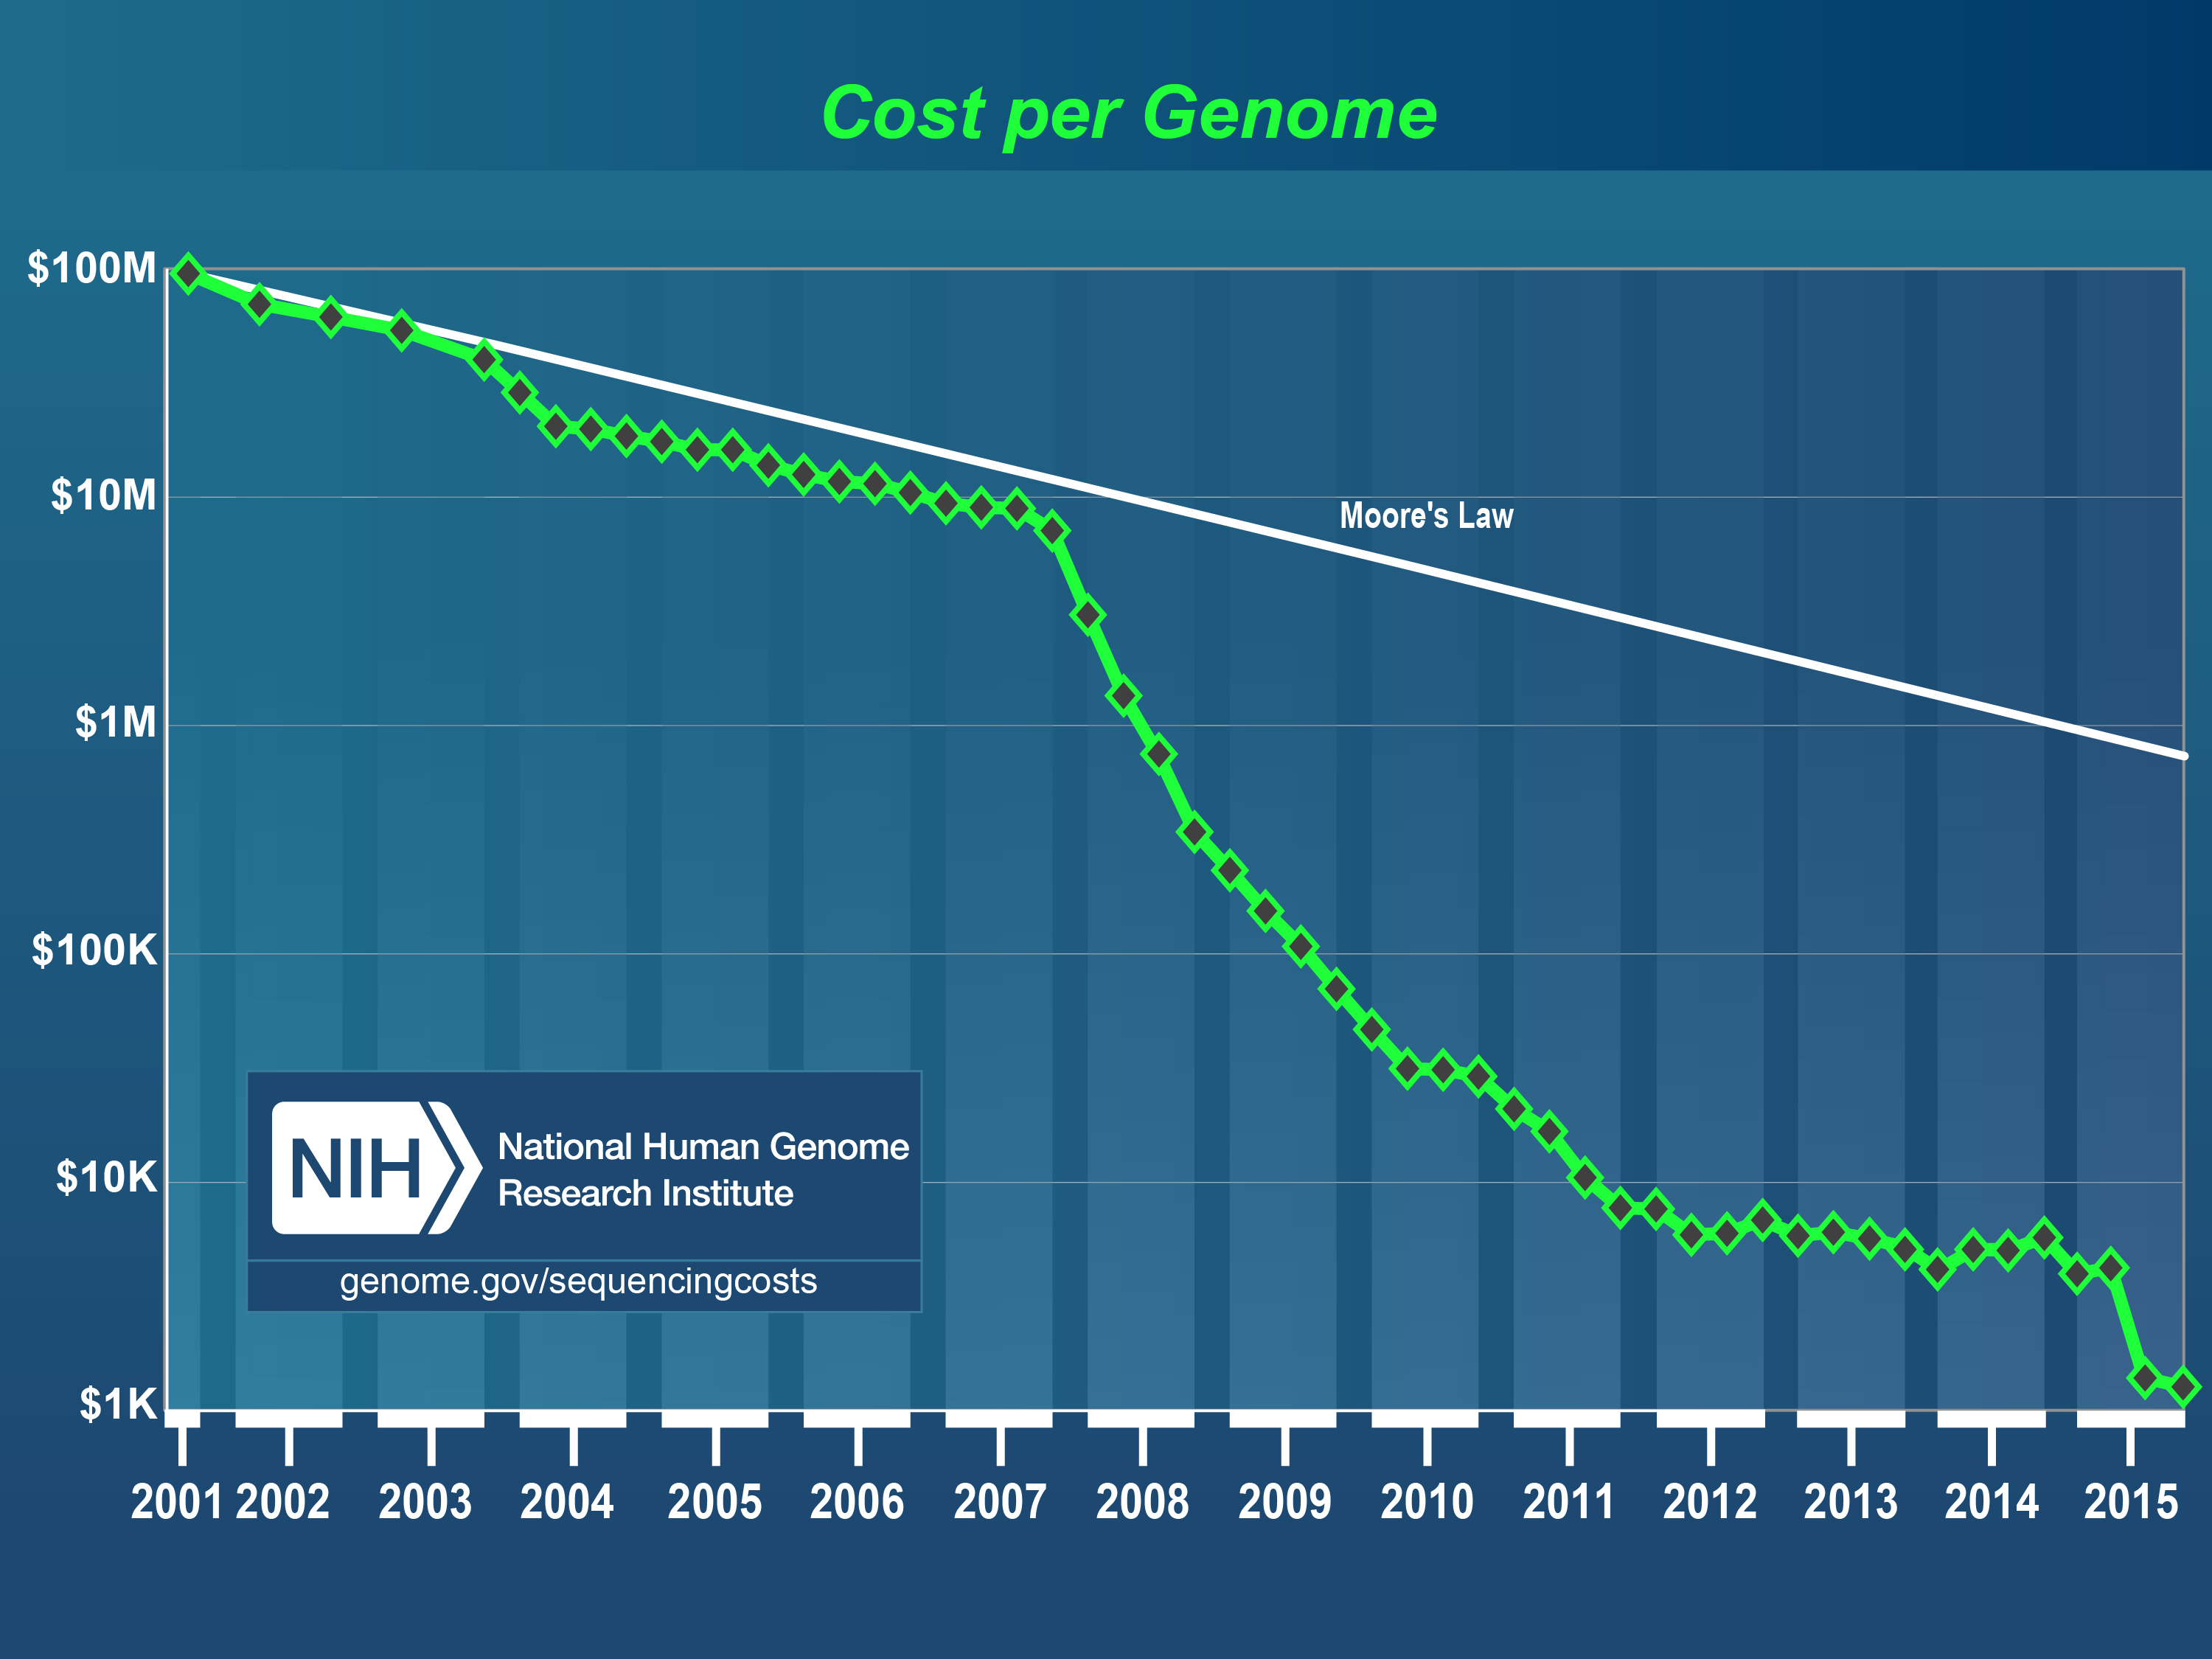
\includegraphics[scale=0.5]{costpergenome2015_4}
\centering
\caption {Cost of DNA sequencing\autocite{The_Cost_of_Sequencing_a_Human_Genome_2016-11-04}}
\label{fig:costpergenome2015_4}
\end{figure}

Figure \ref{fig:costpergenome2015_4} shows the change in the cost of DNA sequencing over the course of the past 15 years. The precipitous drop in sequencing cost observed since 2008 coincides with wide adoption of NGS methodologies. This drop in price has made tractable a new set of large scale genomics sequencing projects that aim to characterize human genetic diversity at population scale, projects such as the 1000 Genomes Project\autocite{10002010map}, and the large scale sequencing of the Icelandic population\autocite{gudbjartsson2015large}.

\subsection{Genomics Studies}

\subsection{Cancer Genomics}
Cancer is a genetic disease that has an extremely high burden on the human population. In 2012, the global incidence of new cases worldwide has been estimated as 14.1 million, and deaths at 8.2 million\autocite{torre2015global}. The economic cost of cancer to the European Union has been estimated at 126 billion euro in 2009\autocite{luengo2013economic}, and in the US \$124.5 billion USD in 2010\autocite{yabroff2011economic}. Because of the genetic nature of the disease studying genomes of cancer patients helps uncover the mechanisms behind the development and evolution of cancer\autocite{stratton2009cancer}.

Cancerous tumours arise from a single cell which over time accumulates a series of somatic mutations that cause it to exhibit properties such as: increased mutation rate, increased proliferation, anchorage independent growth, and resisting cell death\autocite{hanahan2011hallmarks} . Only certain mutations, however, contribute to the development of cancer, while others are benign. Cancer genomics studies aim to identify and characterize those mutations that are cancer drivers and play a role in the formation or progression of tumours\autocite{stratton2009cancer}. 

Studying cancer genomes is more complex and expensive than studying the genomes of healthy individuals because each patient requires that two DNA samples are collected - that of the normal tissue, and that of the tumour. This is necessary to identify those mutations that are somatic - i.e. only occur in the tumour cell population\autocite{roberts2013comparative}.


\begin{figure}[H]
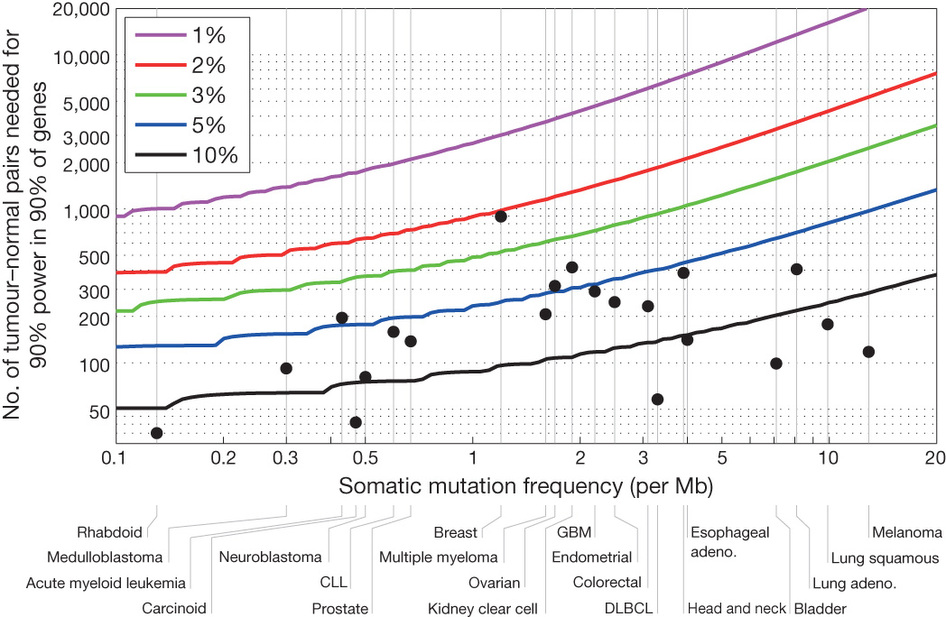
\includegraphics[scale=0.4]{nature12912-f5}
\centering
\caption {Sequencing sample size required by mutation rate\autocite{lawrence2014discovery}.}
\label{fig:nature12912-f5}
\end{figure}

Although there is a large number of identified mutations that are implicated in cancer (2,002,811 SNV,  10,534 gene fusions, 61,299 genome rearrangements, 695,504 CNV segments in COSMIC v70; August 2014)\autocite{forbes2015cosmic}, each mutation has a low chance of being present in any given tumour. Figure \ref{fig:nature12912-f5} demonstrates the sample size required to have 90\% statistical power to identify  90\% of the variants that occur with a set frequency in tumours with varying background mutation rates. Thus, identifying 90\% of the mutations occurring with a frequency of at most 1\% in Lung Adenocarcinoma requires a sample size of at least 10,000 patients. The necessity to sequence large cohorts of patients in order to be able to comprehensively detect  cancer related genomic variants has led to the creation of several large scale cancer sequencing studies.

\subsection{Clinical Genomics}

\section{Computational Methods for Next Generation Sequencing}
Abracadabraca. Because the size of a typical genome is millions to billions of basepairs long, and current DNA sequencing technology frequently generates errors during the sequencing process, requiring multiple samples of each genomic location to be generated, the amount of data required to be examined in order to characterize even a single sample is well beyond the capabilities of any human. Thus, a multitude of computational approaches are required in order to make the task tractable for individual samples as well as cohorts, and entire populations.

The task of comprehensive characterization of genomic data for an individual is typically decomposed into a series of computational steps, each with its own data representation, and typically developed by a separate research group, which are then assembled into computational pipelines and executed by workflow engines on diverse computing environments. Our goal in this section is to enumerate and describe the individual steps and to provide a survey of the key computational tools and data formats that presently form the set of best practices in this rapidly evolving branch of science. Since Rheos is designed to improve upon these best practices we identify in each section the key mathematical and algorithmic ideas that underpin each approach in order to adapt and translate them into the Rheos framework.

The data that is used in virtually all modern genomics studies is generated on a next generation DNA sequencing machine. Several types of sequencers have been developed but the most frequently used ones are made by Illumina. The raw data produced by such a sequencer is a set of image files, where the color of each pixel represents the corresponding nucleotide base in a DNA strand that is being sequenced in each micro-well of a flowcell, representing the sample of interest. The succession of images produced by each cycle of sequencing then results in a set of reads, a collection of randomly ordered DNA fragments that are further analyzed by downstream tools. The first challenge in generating these reads is the accurate interpretation of pixel colors and mapping them to the corresponding nucleotide bases, known as base-calling. Because all of the currently available DNA sequencing methodologies are imperfect at reading the underlying DNA sequence a number of errors is introduced into the process at various stages and special QA software is required in order to detect and assess the location and severity of the errors. A typical output of the QA process is a filtered set of reads where the lowest quality reads have been filtered out and each base within each read is assigned a quality score which represents the best current estimate of the probability that the base has been called incorrectly. The currently most frequently used file format for storing DNA sequence reads along with their read qualities is a text file known as fastq.

Depending on whether the organism under study has previously been sequenced there may already exist a reference sequence for it i.e. a file that for each genomic location describes the most frequently occurring nucleotide for that species at that location. Humans, and many other species of organisms already have reference sequences available. If the reference sequence for the organism under study is available then the next processing step involves searching for the position in the reference sequence that best matches each read that has been generated for the sample under study in the previous step. The coordinate of the best match is then assumed to be the location in the genome where that particular read has originated from. This process is known as genome alignment and it is very resource intensive for species with large genomes such as humans (~3 billion bases) because a typical sequencing effort will generate at least ~1 billion reads for a single sample, and each read needs to be mapped to the reference genome. This problem is made more difficult by the fact that an organism's genome typically has a large proportion of repeated sequence fragments and thus the generated reads do not uniquely align to a single location on the reference. A list of matching positions is generated instead, where each match needs to be scored and the highest scoring match is assumed to be the true origin of the read. Many alignment algorithms exist but the most accurate and fast ones use a two step process of indexing, implemented via hash tables or prefix/suffix tries, to generate a short list of promising match locations, followed by a more exact local alignment that uses dynamic programming to generate a best match. The alignment process is further complicated by the presence of sequencing errors, various genomic variants, and disease state such as cancer, all of which generate significant (and sometimes drastic) differences between the obtained reads and the reference genome, thus necessitating inexact matching approaches. The best algorithms that are currently available have a typical runtime of 24-48 hours on a modern 8-core machine. The most widely adopted standard for storing the alignment data on disk is the SAM\autocite{li2009sequence} (and its binary and indexed counterpart BAM) format developed in the context of the 1000 Genomes Project. In addition to the sequence data and base qualities that are already available in fastq, the SAM format adds a reference coordinate to each read, an overall mapping quality for the read, and whether each position in the read matches the reference sequence, along with other useful metadata. 

When a reference sequence does not exist, or when it is undesirable to use one, genome alignment tools are inapplicable and a different approach, called de-novo assembly, is used. Under this approach each read is broken into smaller subsequences called k-mers (of length k), these k-mers are then used to build a graph structure called a de Bruijn graph. Unique paths through the graph represent possible arrangements of reads that correspond to the underlying sequence and the highest scoring path is chosen as the true sequence. Using the de-novo assembly approach has some advantages over alignment-based methods because it models the structure of the organism's genome directly as it is observed rather than in relation to a reference. This is because no reference is perfect, but instead each reference has its own set of errors that were introduced in its construction. Furthermore, genomic structural variants, which represent large (hundreds to millions of basepairs long) sequences that may be deleted, duplicated, or inverted within a given genome challenge alignment software because of the alignment errors that they introduce and require sophisticated algorithms to later detect, whereas in the de-novo assembly approach these variants are directly modelled as they occur in the underlying sequence and are thus easier to identify. De-novo assembly has its own set of challenges however related to difficulties dealing with repetitive sequences that are found within the genome, as well as the extremely high resource requirements of de-novo assembly algorithms, especially when it comes to memory. The de Bruijn graph is typically built in memory and can be multiple terabytes in size, thus requiring computers with extremely high memory to process. Since, even when using in-memory graph construction the runtime for a single sample is typically several days, it is impractical to move the graph representation to disk without dramatically increasing the algorithm runtime to the point where its duration becomes unreasonable. In practice whole genome de-novo assembly is currently rarely used for processing human genomic data because of the challenges described above. Instead, modern algorithms supplement read alignment with local assembly of particular genomic regions of interest in order to reap some of the benefits offered by assembly-based methods without incurring all of the costs. 

Once the reads have been aligned they are typically sorted by genomic coordinate so that all of the reads that overlap a given coordinate can be examined together at once. This is an expensive sortation step that does not lend itself well to parallelization and takes several hours to complete per sample. Subsequent to the sortation step is another round of data QA which aims to throw out low quality reads that poorly align to the reference. Care must be taken however, because these low quality reads may not only signal underlying data or sequencing issues like sample contamination, or lane-swap, but may also signal the presence of structural variants or integration of retrovirus DNA into the host under study, both of which are of high interest to properly identify. Thus, it is common to split the sample into reads of high quality that are further assessed with one set of algorithms and a set of reads that map with low quality, or fail to map at all, to be assessed with a different set of algorithms.

At this point the data is ready to begin the process of variant calling, that is, identifying the genomic features of the sample that are different from the reference sequence for that organism (i.e. mutations). It is important to distinguish germline variant calling from somatic variant calling at this time. In germline variant calling we are trying to identify the set of variants that have been passed to the individuals under study from their parents and are thus present in every cell of the organism forming the underlying genetic background of that individual where some variants may be neutral to the organism's survival, some may be beneficial, and some may be deleterious. Comprehensively identifying and classifying these is of significant research and clinical interest as they confer susceptibility or resistance to certain disease vectors as well as potential medical remedies and may act as biomarkers to predict disease prognosis or response to treatment within the groups of patients that harbour them.

Somatic mutations are those that each individual cell accumulates over its lifetime and they are of especial interest in the context of cancer where a certain set of mutations accumulated in a particular sequence and over a period of time disrupt the normal cell lifecycle and result in the formation of a malignant tumour. In this context researchers typically sequence both healthy cells (such as those drawn from the patient's blood) and cancerous cells. Mutations are identified in both and the difference between these sets of mutations is then stipulated to be the set of somatic mutations present within that tumour. Just like in the germline case, not all of the somatic mutations contribute to the formation of the cancer and the appropriate identification and classification of those mutations that do (so-called cancer drivers) is an important question of significant clinical and research importance which we consider further below. From a technical standpoint calling somatic variants is significantly more complex than calling germline variants because healthy cells generally conform to the underlying genetic characteristics of the organism, such as the number of chromosomes and ploidy (23 chromosomes, diploid, for humans), whereas in the cancer cells these characteristics can be severely disrupted with entire chromosomes missing or present in amplified copy number, requiring different and more complex statistical models to accurately identify. An additional complexity that is unique to somatic variant calling is the concept of sub-clonal mutations. These are mutations that have been acquired only by some of the cells within a tumour. Since sequencing samples data from a large number of cells within a tumour the reads from which are all pooled together, only a comparatively low number of reads will contain information about sub-clonal mutations, thus making them more difficult to detect, even though such mutations may have a significant impact on the tumour phenotype and thus would be very important to properly identify.

We typically think of three classes of genomic variants that are identified by different methods and oftentimes by separate tools. The simplest to accurately detect, and most frequently occurring are Single Nucleotide Polymorphisms (SNPs), in the germline case, and Single Nucleotide Variants (SNVs), in the somatic case. These are single basepair substitutions where the germline genome differs from the reference sequence by a single letter (for SNPs), or the somatic genome differs from the germline genome by a single letter (for SNVs). SNPs are quite common in humans and occur at the rate of approximately 1 per 1,000 bases on average, or, equivalently, 3 million per individual. Somatic SNVs have a widely varying incidence rate depending on the type of cancer involved with typical rates between (INSERT RATES HERE). For humans, which are diploid (i.e. have two copies of each of the chromosomes, except for the sex chromosomes X and Y), we classify SNPs and SNVs as being either heterozygous (with one reference allele and one variant allele) or homozygous (with both alleles being variant). Methods to detect and accurately genotype SNPs and SNVs typically rely on counting the reads that overlap a given genomic position and evaluating a statistical model that contrasts the probability of the site being reference versus the probability of the site being variant in the face of potential sequencing errors which are expressed as base quality scores and mapping quality scores (as previously described). The models employed for somatic SNV detection and genotyping are significantly more complex than the models for germline variant detection because of the possibility of sub-clonal mutations (as previously described) as well as regions of amplified copy number (i.e. regions where the organism is no longer diploid but can have any number of additional copies of a chromosomal region, or an entire chromosome). More advanced methods output not only lists of variant sites for a sample but calculate a distribution of genotype likelihoods, i.e. all the possible genotypes at a given variant site along with their relative probabilities so that these can be integrated into the models of downstream statistical analyses in a comprehensive manner.

Indels represent sequence insertions and deletions that are anywhere from 1 basepair (bp) to about 50 basepairs long. There is no strict upper bound on the length of an indel and individual tools typically decide on their own cutoffs for length although pretty much all tools place their cutoff at a length that is smaller than the typical read length (150 - 500 bp presently). Indel callers typically look for several mismatched bases in a row between the reference and the sample under study and classify the entire length of the mismatched sequence as an insertion or deletion correspondingly. Other indel callers borrow some of the methodology from structural variant callers which are similar to indels, only typically bigger in size, and are potentially more complex.

Structural variants (SVs) are more large scale genomic rearrangements that occur in both germline and somatic genomes and can have a very drastic effect on the organism's phenotype because they can affect a large number of genes at once, resulting in the loss of function of particular important genes, or the creation of gene fusions where, because of a rearrangement, one gene comes under the programmatic control of another gene thereby disrupting important cellular processes. The most common types of structural variants include insertions, deletions, segmental duplications, inversions, and translocations. Simpler structural variants sometimes combine to produce more complex events that are especially difficult to detect properly. The methods for calling and genotyping of structural variants typically rely on looking at the reads that are deemed low quality for the SNP calling process. These are reads that fail to map to the reference genome, split-reads, which are reads where one part of the read maps to one location on the reference and another part of the read maps to another location, and divergently mapped reads (sequencing is frequently done on read pairs where two ends of a DNA fragment of standard size are sequenced in the opposite directions generating a pair of reads with a standard distance, called insert size, inbetween them), with a shorter or longer than expected insert size. SV callers break down these reads into smaller fragments (k-mers) and attempt to map these k-mers to the reference sequence. The goal is to determine the location of breakpoints, which are positions on the sample genome where a DNA strand break is thought to have occurred as part of the genomic rearrangement that has taken place. Once a list of breakpoints is obtained the algorithm attempts to reconstruct the most likely event sequence that these breakpoints could have arisen from, pairing up adjacent breakpoints that are the result of a sequence deletion, for example. Thus, each pair of breakpoints typically gives rise to a single SV call in the final output of the caller. SV calling is a complex and error-prone process that generates double-digit false-positive and false-negative rate, especially in the somatic case, where patient genomes can undergo drastic rearrangements as a result of cancer-related processes such as chromothripsis and are thus extremely difficult to resolve with accuracy.

Once variants (SNPs/SNVs, Indels, and SVs) have been comprehensively called, a filtering step is necessary because callers are typically initially tuned for highest sensitivity in order to detect the most variants, thus admitting an increased number of false positive calls. Additionally, because calling of SNPs and SVs typically occurs separately by different tools there can be significant call-set overlap where the SNP caller sees a region as a group of SNPs, whereas the SV caller will see it as a single breakpoint. These overlaps need to be resolved in order to avoid redundant calls. A number of filtering approaches exist, some of which rely on heuristics such as strand bias, or read support to filter out low quality variants. Other filtering approaches rely on curated variant databases or machine learning methods in order to reduce the number of false positive calls. One popular filtering approach involves ensemble calling where several different variant calling methods are used on the same dataset and a variant is excluded unless it is called by multiple tools. These methods are typically able to reduce the false positive rate of the call-set by 5-10\% while only nominally affecting the false negative rate.

When a filtered high quality call-set has been prepared it is of interest to determine which of the variants are likely to have an effect on the organism's phenotype and which variants are likely to have no consequence. This is accomplished via variant annotation. The annotation process consults a database of known genes and other genomic elements (promoters, enhancers, etc.) to determine the likely consequence of each variant based on the type of mutation that it represents i.e. a synonymous mutation (that doesn't change the underlying amino acid) is likely to have no phenotypic effect, whereas a stop gain mutation inside the coding region of a known gene may indicate a potential loss of function of that gene and may thus have a considerable effect on the observed phenotype. When annotating somatic mutations it is important to consider known cancer genes and delineate whether mutations are "passengers" or "drivers" depending on whether they are thought to be driving the carcinogenesis process by constitutively activating a cancer gene or deactivating a tumour suppressor, or they are simply acquired as part of the genomic instability that is induced by carcinogenesis. An outcome of the variant annotation process then, is a list of somatic or germline variants accompanied by a designation of the known genomic features that they fall in, along with an assigned functional impact. This is typically the last step of an NGS analysis pipeline after which the variant call-set is considered completed and can be used for any number of downstream analyses depending on the particular research question or clinical application being considered. For instance, the variants may be used as input into a Genome Wide Association Study (GWAS), a Quantitative Trait Locus (QTL) analysis, a rare variant association study, or as input into the computation of a clinical biomarker. 

\subsection{File Formats}
FASTQ - 
BAM/SAM -
CRAM -
VCF - 

\subsection{Base-calling}

\subsection{Alignment}
BWA/MEM -
Bowtie - 
Gem - 

\subsection{Raw Data QA}

\subsection{Germline SNP Calling}
samtools - 
freebayes - 
GATK - 
Platypus


\subsection{Germline Indel Calling}

\subsection{Germline Structural Variant Calling}
Delly - 
Hydra - 


\subsection{Variant Filtering}

\subsection{Somatic SNP Calling}
Mutect - 
Muse - 
Pindel -


\subsection{Somatic Indel Calling}

\subsection{Somatic Structural Variant Calling}

\subsection{Germline Variant Annotation}
Annovar - 
Variant Effect Predictor - 


\subsection{Somatic Variant Annotation}

\subsection{de-novo Assembly}
Velvet -
Abyss - 

\section{Service Oriented Architectures}

\section{Stream-based Systems}

